\documentclass[10pt,a4paper]{article}
\usepackage[utf8]{inputenc}
\usepackage[french]{babel}
\usepackage[T1]{fontenc}
\usepackage{amsmath}
\usepackage{amsfonts}
\usepackage{amssymb}
\usepackage{graphicx}
\usepackage{fullpage}

\title{Comment supprimer le grillage sur des photos de zoo\\ Rapport intermédiaire}
\author{Vincent Bodin \& Vincent Roulet}
\date{4 Avril 2014}


\begin{document}
\maketitle
\hrulefill

\section{Présentation du projet}
Notre projet consiste à chercher à supprimer le grillage des photos de zoo. Pour cela il se sépare en quatre étapes :
\begin{enumerate}
\item Extraction de descripteurs pertinents pour reconnaître les lignes du grillage
\item Détection des lignes du grillage à l'aide de la transformée de Hough
\item Création d'un masque correspondant au grillage
\item Récupération de l'image sans le grillage à l'aide de méthodes d'intpainting
\end{enumerate}

Si la démarche semble théoriquement simple, elle se heurte à de nombreux problèmes pratiques, les photographies de zoo avec grillage sont en effet bien différentes les unes des autres. Un descripteur seul ne suffit donc pas si l'on veut optimiser la tâche. En outre il s'agit de reconnaître non seulement des lignes mais une structure plus riche qu'est le grillage.

Le masque peut être aisément extrait une fois les lignes reconnues. Nous utiliserons les techniques d'inpainting vues dans le cours de Gabriel Peyré du MVA dont les ressources sont en ligne pour réaliser la reconstruction de l'image.

\section{Plan du projet}
\subsection{Extraction de descripteurs}
Nous avons cerné de nombreux descripteurs à combiner ensemble pour donner en entrée de la transformée de Hough.

\paragraph{Canny edge detecteur. }Nous utilisons tout d'abord les contours trouvés à l'aide de la méthode de Canny dont nous prenons des paramètres automatiquement.

\paragraph{K-means couleur. }A l'aide d'un K-means couleur nous détectons la variation de couleur trouvée dans un contour par la méthode de Canny. Le grillage a en effet le plus souvent qu'une ou deux couleurs dans la photographie.

\paragraph{Transformée de Fourier. }La transformée de Fourier de l'image révèle la structure périodique du grillage et peut être ainsi être combinée afin de connaître les orientations pertinentes des contours. Bien qu'elle semble redondante par rapport au post-traitement possible après la transformée de Hough, cette information peut permettre d'affiner les lignes trouvées précédemment. Une alternative pourrait aussi de travailler directement sur la transformation de Fourier : les hautes fréquences sont en effet quasi uniquement présentes dans le grillage et de plus le maillage du grillage est représenté par une "croix" en Fourier (si les orientations étaient parfaites : un ensemble de croix pour des images dont le côté orthogonal du grillage aurait été altéré par une transformation homothétique).

\paragraph{Transformations morphologiques. }Nous avons essayé d'extraire le gradient morphologique afin de comparer son résultat avec celui trouvé par la méthode de Canny. Là encore l'information est redondante mais pourrait affiner les résultats dans le cas d'une photographie "difficile".

Nous avons aussi essayé le chapeau haut de forme. Cependant celui-ci nécessite l'utilisation d'un élément structurant adapté, de simples boules n'apportent en effet pas d'information. On peut donc penser à détecter des croisements de segments à l'aide de cette transformée morphologique.

\subsection{Détection des lignes}
\paragraph{Transformée de Hough. }La transformée de Hough nous permet de détecter les lignes de l'image à l'aide des descripteurs donnés en entrée de cette transformation. Le paramètre de sélection de ces lignes reste à optimiser (quel score minimum faut-il pour qu'une ligne soit prise ne compte ?)

\paragraph{Post-traitement de la transformée de Hough. }Comme dit précédemment un grillage a une structure plus riche qu'un simple ensemble de lignes : les lignes trouvées par la transformée de Hough doivent être parallèles ou faire un angle d'environ $90$\degre $\pm 10$\degre. Cette information permet de filtrer les lignes perçues précédemment.

\subsection{Extraction d'un masque}
Pour extraire le masque il s'agit de prendre une zone autour de chaque ligne, réaliser un K-means couleur et ne garder que les zones à faible variance colorimétrique dans la base décrite par le K-means couleur.

\subsection{Inpainting}

Nous avons retenu principalement trois méthodes d'inpainting dont deux nous semblent intéressantes pour ce projet.

\paragraph{Inpainting avec régularisation variationnelle. }Nous allons essayer d'effectuer de l'inpainting avec des méthodes de régularisation variationnelle, les approches traditionnelles étant celles de Sobolev et celle de la norme TV. 

\paragraph{Inpainting avec régularisation parcimonieuse. }L'idée serait de tester l'effet d'un algorithme \emph{forward-backward} et d'effectuer l'inpainting avec une base d'ondelettes orthogonales. Le cas particulier des ondelettes invariantes aux translations donne souvent un excellent SNR et une rendu visuel joli.

\paragraph{Inpainting par projection de patch. }Cette méthode est surtout utilisée pour synthétiser des textures. Nous ne savons pas encore si elle s'applique bien à notre cas.


\section{Travail passé et futur}
\subsection{Travail déjà effectué}
\paragraph{Extraction de descripteurs. } Nous avons déjà extrait les descripteurs décrits ci-dessus en les essayant un par un pour observer les lignes détectées. Nous essayons actuellement de les combiner afin d'obtenir une entrée correcte pour la transformée de Hough.

\paragraph{Détection de lignes. } Nous avons tenté une transformée de hough sur la transformée de Hough afin de détecter les lignes parallèles. Les résultats n'étaient pas encore très concluants notamment parce que nos descripteurs n'étaient pas assez pertinents. En figure \ref{hough} est représenté une extraction de lignes à l'aide uniquement des contours trouvés par la méthode de Canny.

\begin{figure}[ht!]
\begin{center}
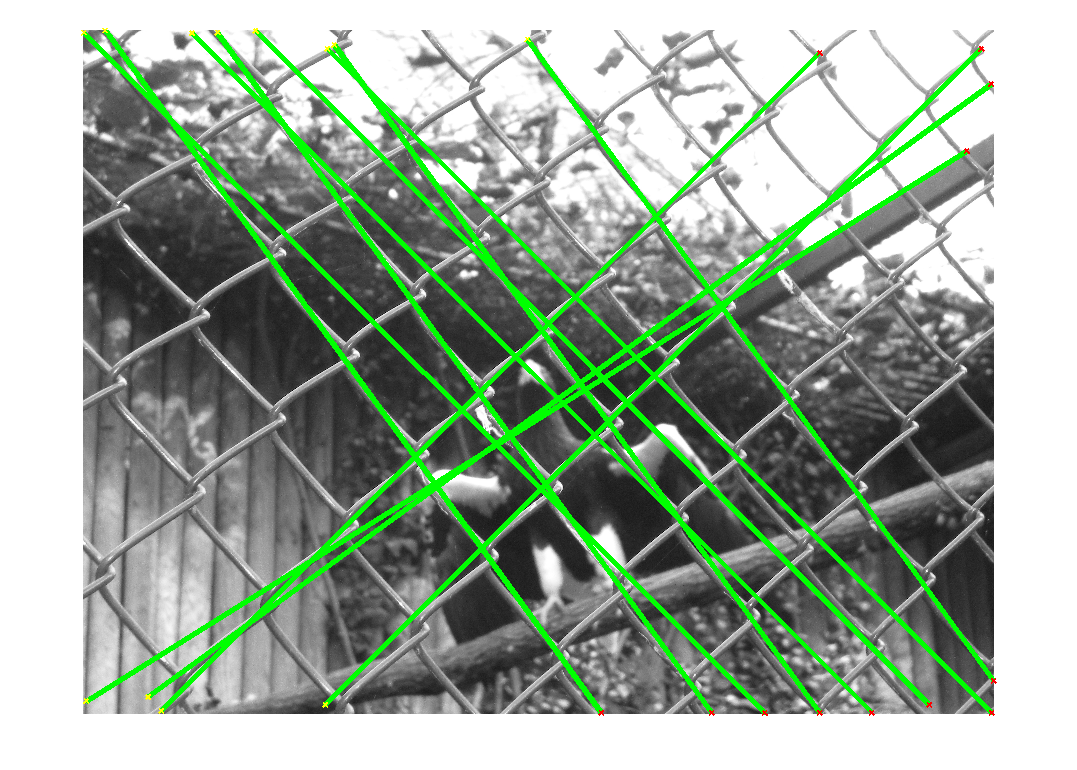
\includegraphics[scale=0.3]{fig/hough.png}
\caption{\label{hough}Extraction de lignes à l'aide uniquement des contours trouvés par la méthode de Canny}
\end{center}
\end{figure}

\paragraph{Extraction du masque. } N'ayant pas encore un grillage correct nous n'avons pas encore pu extraire de masque bien que nous avons une bonne idée de la façon de l'extraire.

\paragraph{Inpainting} Celui-ci interviendra après l'extraction de masque. Les algorithmes ont déjà été codés pour la plupart pour autant et fonctionnent sur des masques aléatoires.

\subsection{Travail futur}
Nous aimerions achever la démarche décrite précédemment afin de la tester sur des photos que nous prendrions nous-même. S'il nous reste du temps nous comparerons les résultats obtenus avec ceux des articles \cite{YLiu2008}.

\bibliographystyle{unsrt}
\bibliography{Bib}

\end{document}